\documentclass[12pt]{article}
\setlength{\oddsidemargin}{0in}
\setlength{\evensidemargin}{0in}
\setlength{\textwidth}{6.5in}
\setlength{\parindent}{0in}
\setlength{\parskip}{\baselineskip}

\usepackage{amsmath,amsfonts,amssymb,graphicx, hyperref, float}

\begin{document}

IBEHS 4A03 \hfill Assignment \#3\\
Baoze Lin, Hady Ibrahim

\hrulefill

% Custom numbering for subparts (e.g., 2.1, 2.2)
\renewcommand{\theenumii}{\arabic{enumi}.\arabic{enumii}}

\begin{enumerate}
\item Question 1
  \begin{enumerate}
    % Answer to 1.1
    \item
    The open-loop step response of the system is shown in the Simulink model (Figure \ref{fig:figure1_1}) below with the response shown in Figure \ref{fig:figure1_2}.
    
    \begin{figure}[H]
      \centering
      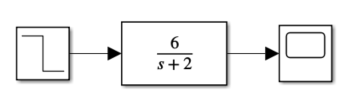
\includegraphics[width=0.3\textwidth]{Figures/Models/model1_1.png}
      \caption{Simulink model of the open-loop step response}
      \label{fig:figure1_1}
    \end{figure}

    \begin{figure}[H]
      \centering
      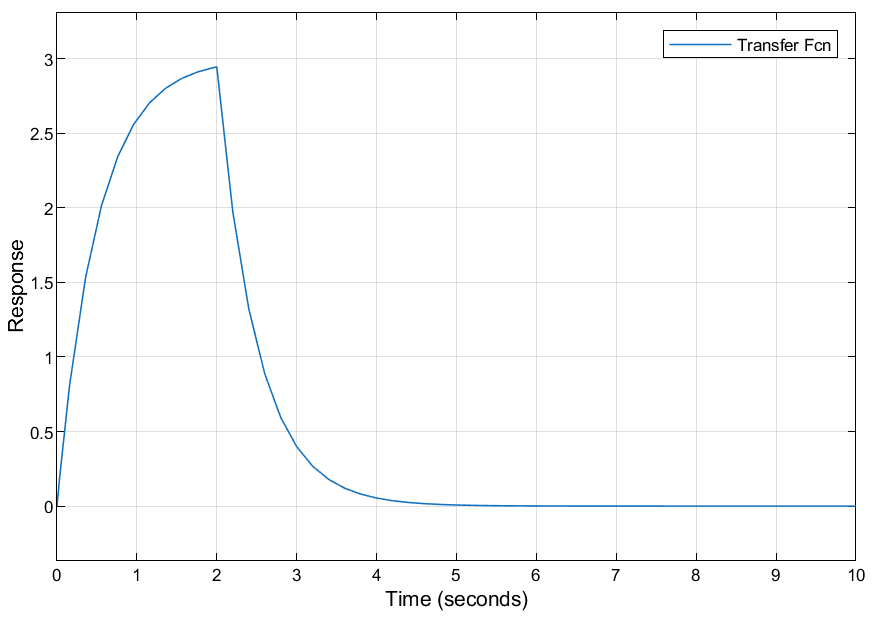
\includegraphics[width=0.5\textwidth]{Figures/figure1_1.png}
      \caption{Open-loop step response}
      \label{fig:figure1_2}
    \end{figure}

    To identify the gain and time constant for this system, we can rearrange the transfer function to isolate the gain K and time constant $\tau$:

    The given transfer function is:
    \[
    G_p(s) = \frac{6}{s + 2}
    \]

    To express this in the standard first-order form, which is:
    \[
    G(s) = \frac{K}{\tau s + 1}
    \]
    where \( K \) is the gain and \( \tau \) is the time constant.

    We rearrange \( G_p(s) \) as follows:
    \[
    G_p(s) = \frac{6}{2(\frac{1}{2}s + 1)} = \frac{3}{\frac{1}{2}s + 1}
    \]

    Thus, we identify the gain \( K \) and the time constant \( \tau \) as:
    \[
    K = 3, \quad \tau = \frac{1}{2}
    \]

    % Answer to 1.2
    \item 
    The closed-loop feedback control with a proportional controller is shown below in Figure \ref{fig:figure1_3}. The transfer function $G_c(s)$ can also be represented by a proportional gain $K_c$.

    \begin{figure}[H]
      \centering
      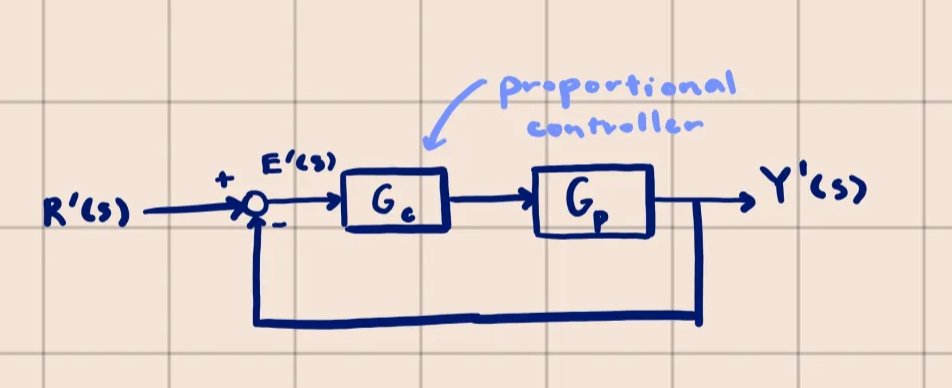
\includegraphics[width=0.7\textwidth]{Figures/Models/model1_2.png}
      \caption{Simulink model of the closed-loop feedback control with a proportional controller}
      \label{fig:figure1_3}
    \end{figure}
    
    \pagebreak
    
    % Answer to 1.3
    \item 
    The Simulink model is shown below in Figure \ref{fig:figure1_4}. The response of the system is shown in Figure \ref{fig:figure1_5}.

    \begin{figure}[H]
      \centering
      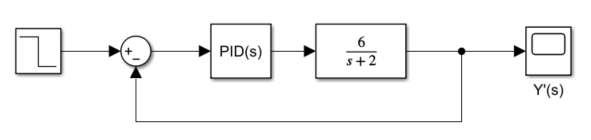
\includegraphics[width=0.7\textwidth]{Figures/Models/model1_3.png}
      \caption{Simulink model of the closed-loop feedback control with a proportional controller}
      \label{fig:figure1_4}
    \end{figure}

    \begin{figure}[H]
      \centering
      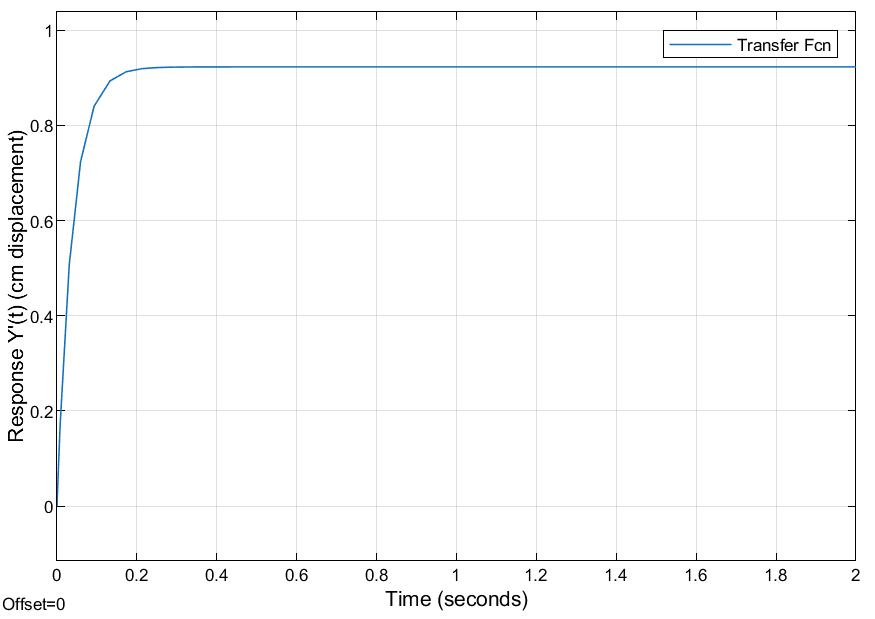
\includegraphics[width=0.8\textwidth]{Figures/figure1_3.png}
      \caption{Closed-loop step response}
      \label{fig:figure1_5}
    \end{figure}

    % Answer to 1.4
    \item
    The closed-loop transfer function \( T(s) \) is given by:
    \[
    T(s) = \frac{Y'(s)}{R'(s)} = \frac{G_c(s)G_p(s)}{1 + G_c(s)G_p(s)}
    \]

    Where \( G_c(s) = K_c = 4 \) (proportional controller) and \( G_p(s) = \frac{6}{s+2} \) (plant transfer function). Substituting the transfer functions:
    \[
    T(s) = \frac{4 \cdot \frac{6}{s+2}}{1 + 4 \cdot \frac{6}{s+2}}
    \]

    Simplifying:
    \[
    T(s) = \frac{\frac{24}{s+2}}{1 + \frac{24}{s+2}} = \frac{24}{s+2+24} = \frac{24}{s+26}
    \]

    Thus, the closed-loop transfer function is:
    \[
    T(s) = \frac{24}{s+26}
    \]

    We then apply the Final Value Theorem, which states that:
    \[
    \lim_{t \to \infty} y(t) = \lim_{s \to 0} sY(s)
    \]

    For a unit step input \( R'(s) = \frac{1}{s} \), the Laplace transform of the output is:
    \[
    Y'(s) = T(s)R'(s) = \frac{24}{s+26} \cdot \frac{1}{s}
    \]

    Applying the FVT:
    \[
    \lim_{t \to \infty} y(t) = \lim_{s \to 0} s \cdot \frac{24}{(s+26)s} = \lim_{s \to 0} \frac{24}{s+26} = \frac{24}{26} = \frac{12}{13} \approx 0.923
    \]

    The steady-state value of the output is approximately \( 0.923 \). Since the system is operating on displacement from a rock assembly, the set point is 0. Thus, the offset of this system is approximately \( 0.923 \). Referring to the step response in Figure \ref{fig:figure1_5}, we can see the offset is approximately \( 0.923 \).

    % Answer to 1.5
    \item
    THe closed-loop system for controller gains $K_c = {0.25, 1, 2, 4, 10}$ are shown in Figure \ref{fig:figure1_6}. Observing the results, we can see that the offset of the system decreases as the proportional gain increases.

    \begin{figure}[H]
      \centering
      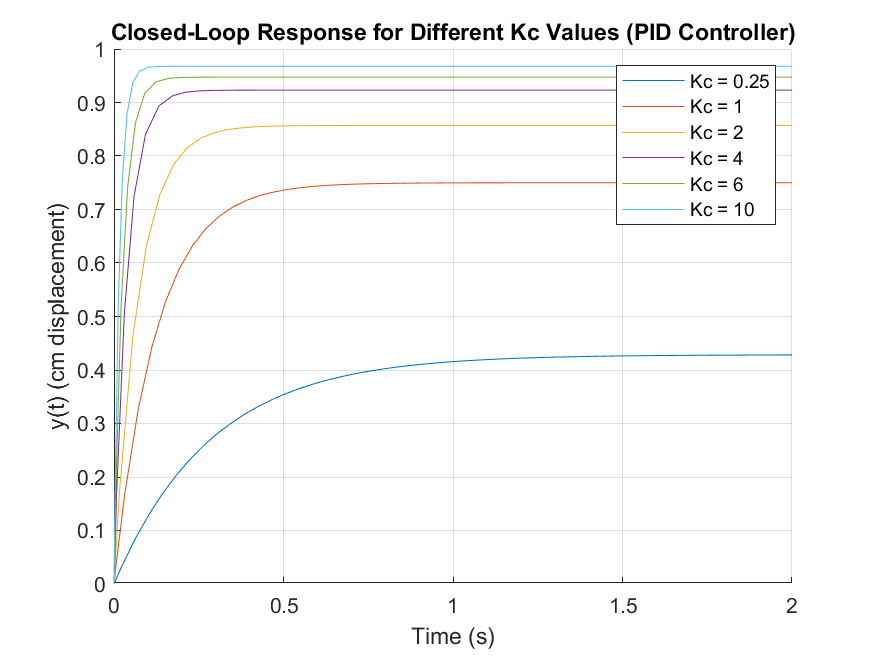
\includegraphics[width=0.8\textwidth]{Figures/figure1_5.png}
      \caption{Closed-loop step response for different controller gains}
      \label{fig:figure1_6}
    \end{figure}

  \end{enumerate}

\pagebreak

\item Question 2
  \begin{enumerate}
    \item placeholder
  \end{enumerate}

\end{enumerate}

\end{document}
